% \vspace{-3ex}
\begin{figure}[h]
\centering
% \cfbox{box-gray}{
\resizebox{!}{0.25\columnwidth}{
% \tikzsetnextfilename{}
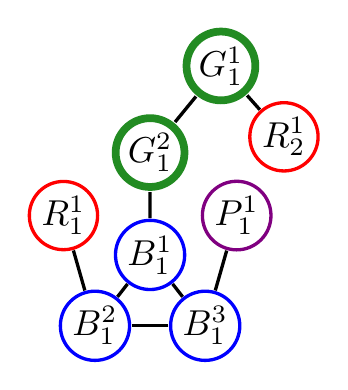
\begin{tikzpicture}[
mynode/.style={draw, circle, very thick, inner sep=1pt, scale=1.3},
myline/.style={draw, very thick},
]

\node[mynode,draw=red] (1) at (1.7,0) {$\xcolor{R}^1_2$};
\node[mynode,draw=ForestGreen,line width=2.8pt] (2) at (0,-0.2)  {$\xcolor{G}^2_1$};
\node[mynode,draw=ForestGreen,line width=2.8pt] (8) at (0.9,0.9)  {$\xcolor{G}^1_1$};

\node[mynode,draw=blue] (3) at (0,-1.5)  {$\xcolor{B}^1_1$};
\node[mynode,draw=blue] (6) at (-0.7,-2.4)  {$\xcolor{B}^2_1$};
\node[mynode,draw=blue] (7) at (0.7,-2.4)  {$\xcolor{B}^3_1$};


\node[mynode,draw=Purple] (4) at (1.1,-1.0) {$\xcolor{P}^1_1$};
\node[mynode,draw=red] (5) at (-1.1,-1.0)  {$\xcolor{R}^1_1$};

\draw [myline] (1) -- (8);
\draw [myline] (2) -- (3);
\draw [myline] (7) -- (4);
\draw [myline] (6) -- (5);

\draw [myline] (6) -- (7);
\draw [myline] (3) -- (6);
\draw [myline] (3) -- (7);

\draw [myline] (2) -- (8);

\end{tikzpicture}
}
\resizebox{!}{0.1\columnwidth}{

\begin{tikzpicture}
\node[] () at (0,-0.5)  {\scalebox{2}{$\Leftrightarrow$}};
%\node[] () at (0,0.5)  { };
%\node[] () at (0,-1.5)  { };
\end{tikzpicture}
}
% }
% \cfbox{box-gray}{
\resizebox{!}{0.25\columnwidth}{
% \tikzsetnextfilename{}
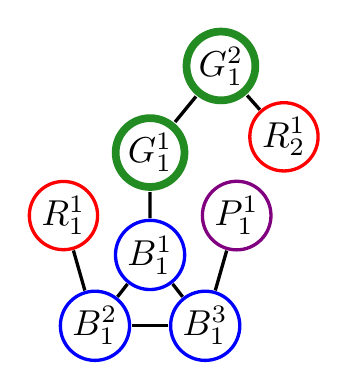
\begin{tikzpicture}[
mynode/.style={draw, circle, very thick, inner sep=1pt, scale=1.3},
myline/.style={draw, very thick},
]

\node[mynode,draw=red] (1) at (1.7,0) {$\xcolor{R}^1_2$};
\node[mynode,draw=ForestGreen,line width=2.8pt] (2) at (0,-0.2)  {$\xcolor{G}^1_1$};
\node[mynode,draw=ForestGreen,line width=2.8pt] (8) at (0.9,0.9)  {$\xcolor{G}^2_1$};

\node[mynode,draw=blue] (3) at (0,-1.5)  {$\xcolor{B}^1_1$};
\node[mynode,draw=blue] (6) at (-0.7,-2.4)  {$\xcolor{B}^2_1$};
\node[mynode,draw=blue] (7) at (0.7,-2.4)  {$\xcolor{B}^3_1$};


\node[mynode,draw=Purple] (4) at (1.1,-1.0) {$\xcolor{P}^1_1$};
\node[mynode,draw=red] (5) at (-1.1,-1.0)  {$\xcolor{R}^1_1$};

\draw [myline] (1) -- (8);
\draw [myline] (2) -- (3);
\draw [myline] (7) -- (4);
\draw [myline] (6) -- (5);

\draw [myline] (6) -- (7);
\draw [myline] (3) -- (6);
\draw [myline] (3) -- (7);

\draw [myline] (2) -- (8);

\end{tikzpicture}
}
% }
\resizebox{!}{0.17\columnwidth}{
% \tikzsetnextfilename{}
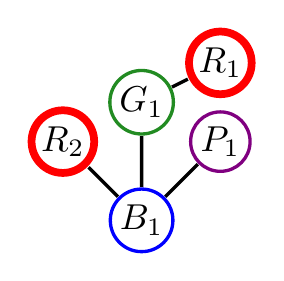
\begin{tikzpicture}[
mynode/.style={draw, circle, very thick, inner sep=1pt, scale=1.3},
myline/.style={draw, very thick},
]
\pgfmathsetmacro{\n}{7};
\pgfmathsetmacro{\r}{1.75};

\node[mynode,draw=red,line width=2.8pt] (1) at (1,0.5) {$\xcolor{R}_1$};
\node[mynode,draw=ForestGreen] (2) at (0,0)  {$\xcolor{G}_1$};
\node[mynode,draw=blue] (3) at (0,-1.5)  {$\xcolor{B}_1$};
\node[mynode,draw=Purple] (4) at (1,-0.5) {$\xcolor{P}_1$};
\node[mynode,draw=red,line width=2.8pt] (5) at (-1,-0.5)  {$\xcolor{R}_2$};

\draw [myline] (1) -- (2);
\draw [myline] (2) -- (3);
\draw [myline] (3) -- (4);
\draw [myline] (3) -- (5);

\end{tikzpicture}
}
\resizebox{!}{0.17\columnwidth}{
\begin{tikzpicture}
\node[] () at (0,-0.5)  {\scalebox{2}{$\Leftrightarrow$}};
\node[] () at (0,0.5)  { };
\node[] () at (0,-1.5)  { };
\end{tikzpicture}
}
% }
% \cfbox{box-gray}{
\resizebox{!}{0.2\columnwidth}{
% \tikzsetnextfilename{}
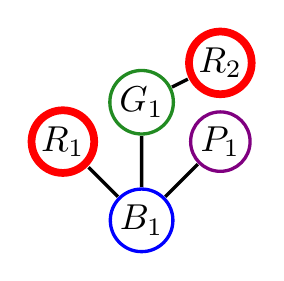
\begin{tikzpicture}[
mynode/.style={draw, circle, very thick, inner sep=1pt, scale=1.3},
myline/.style={draw, very thick},
]
\pgfmathsetmacro{\n}{7};
\pgfmathsetmacro{\r}{1.75};

\node[mynode,draw=red,line width=2.8pt] (1) at (1,0.5) {$\xcolor{R}_2$};
\node[mynode,draw=ForestGreen] (2) at (0,0)  {$\xcolor{G}_1$};
\node[mynode,draw=blue] (3) at (0,-1.5)  {$\xcolor{B}_1$};
\node[mynode,draw=Purple] (4) at (1,-0.5) {$\xcolor{P}_1$};
\node[mynode,draw=red,line width=2.8pt] (5) at (-1,-0.5)  {$\xcolor{R}_1$};

\draw [myline] (1) -- (2);
\draw [myline] (2) -- (3);
\draw [myline] (3) -- (4);
\draw [myline] (3) -- (5);

\end{tikzpicture}
}

\caption{Port-type isomorphism.\label{fig:ch2:piso}}
\end{figure}
% \vspace{-3ex}